%Nome: Guilherme Navarro
%Número USP: 8943160
%Turma: Noturna
%Curso: Laboratório de Computação e Simulação

\documentclass{article} %documento do tipo artigo
\usepackage[brazilian]{babel} %gera datas e nomes como capítulo, bibliografia em português com estilo brasileiro
\usepackage{graphicx} %permite incluir figuras
\usepackage[utf8]{inputenc} %os acentos são digitados diretamente pelo teclado
\usepackage{bbold} %permite escrever os símbolos dos conjuntos
\usepackage{listings}
\usepackage{url}
\usepackage{color}

\begin{document} %início do documento

\title{EP4 - Monte Carlo via Cadeias de Markov (MCMC) - algoritmo de Metropolis-Hastings} %título do documento
\author{Guilherme Navarro - 8943160} %autor do documento
\date{Maio de 2018} %data 

\maketitle

\section{Monte Carlo via Cadeias de Markov}

\qquad O método de Monte Carlo tem se destacado em diversas áreas de estudo devido a sua ampla aplicação. No EP3, foi visto o exemplo de sua utilização em que, a partir do método de simulação via {\it{Importance Sampling}}, é obtida amostra de distribuições a posteriori num único passo. Essa forma de integração é denominado método não iterativo, uma vez que os valores da amostra são gerados de forma independente e não há uma preocupação em relação à sua convergência. 

\ Entretanto, existem vários casos em que as funções de densidade das distribuições de interesse são complicadas e de difícil amostragem. Uma alternativa para isso são os métodos iterativos de Monte Carlo via Cadeias de Markov (MCMC) nos quais, a princípio, obtém-se amostra através de técnicas de simulação iterativa, baseadas em cadeias de Markov ergódicas. Vale ressaltar que, nesses casos, os valores gerados não serão mais independentes, uma vez que a geração do próximo valor da amostra depende de seu valor anterior.

\ O presente relatório tem como objetivo simular o método de MCMC segundo o algoritmo de Metropolis-Hastings.

\section{Constantes utilizadas na simulação}

\qquad Para dar continuidade a simulação do método de integração {\it {importance sampling}}, serão considerados, neste relatório, os seguintes valores: 

\begin{enumerate}
\item $RG = 50057666 \Rightarrow a = 0,50057666$
\item $CPF = 43396344847 \Rightarrow b = 0,43396344847$
\item $NUSP = 8943160 \Rightarrow c = 1,8535791$ 

\end{enumerate}

\section{Algoritmo de simulação}

\ 

\qquad Para a simulação do método de MCMC, considere a seguinte função:

\ $$f(x) = y^{c-1}e^{-y}$$ 

\noindent sendo $y = x + |sin(ax+b)|$, $a = 0.RG$, $b = 0.CPF$ e $c = 1.NUSP$ utilizarei o MCMC para gerar amostras com o intuito de obter uma estimativa do valor de $I$ pelo método iterativo.

\ $$I = \int_{0}^{\infty}f(x) dx $$

\ Utilizando uma função $g(x)$ é uma função de densidade de probabilidade da variável aleatória $X$, então, para gerar uma amostra dessa variável, sendo a seguinte função:

\ $$g(x) = \frac{x^{c-1}e^{-x}}{\Gamma(c)}$$

\ Sabe-se que a variável aleatória $X$, neste caso, possui uma complicada função,  portanto, a geração de sua amostra $x_{1}$, $x_{2}$, ..., $x_{n}$ deve ser realizada a partir de uma amostra $\epsilon_{1}$, $\epsilon_{2}$, ..., $\epsilon_{n}$, da variável aleatória $\varepsilon$ com distribuição do núcleo e com o mesmo domínio $D$ de $X$. 

\subsection{Metropolis-Hastings}

\qquad Para a realização do algoritmo de Metropolis-Hastings, suponha que a  cadeia esteja no estado $x_{i}$ e que $x_{i + 1} = x_{i} + \epsilon_{i}$ é gerado através da distribuição do núcleo. A escolha do próximo valor da amostra é realizada a partir dos seguintes passos:

\begin{enumerate}
\item Especifique o valor inicial $x_{1}$;
\item Gere um valor $\epsilon_{i}$ da distribuição do núcleo;
\item Calcule a probabilidade de aceitação $\alpha(x_{i}, x_{i + 1})$ e gere um valor $u_{i}$ da distribuição Uniforme[0, 1], com

\ $$R(x_{i}, x_{i + 1}) = \frac{g(x_{i + 1})Q(x_{i + 1} - x_{i})}{g(x_{i})Q(x_{i} - x_{i + 1})}$$
\ $$\alpha(x_{i}, x_{i + 1}) = min(1 , R(x_{i}, x_{i + 1}))$$

\item Se $u_{i} \leq \alpha(x_{i}, x_{i + 1})$, então aceite o novo valor $x_{i + 1} = x_{i} + \epsilon_{i}$, caso contrário, $x_{i + 1} = x_{i}$, ou seja

\ $$x_{i + 1} = \left\{ \begin{array}{ll}
x_{i} + \epsilon_{i} & \mbox{ se } u_{i} \leq \alpha \\
x_{i} & \mbox{ se } u_{i} > \alpha \end{array} \right.\ $$

\item Volte ao passo 2.
\end{enumerate}

\ Nota-se que o valor de $Q(x_{i + 1} - x_{i})$, neste caso, é equivalente a $Q(x_{i} - x_{i + 1})$, já que as distribuições do núcleo (normal e uniforme) são simétricas, portanto, o calculo de $R(x_{i}, x_{i + 1})$ pode ser simplificado para

\ $$R(x_{i}, x_{i + 1}) = \frac{g(x_{i + 1})}{g(x_{i})}$$

\ Assim, com esse procedimento, a amostra de $X$ pode ser obtido. No entanto, uma questão importante de ordem prática é como os valores iniciais influenciam o comportamento da cadeia. É importante que, conforme o número de iterações aumenta, a cadeia esquece gradualmente os valores iniciais e eventualmente converge para uma distribuição de equilíbrio. Com isso, em termos práticos, é comum gerar várias amostras de $X$ e selecionar sempre o último valor delas para compor a amostra final da variável $X$.

\ Compreende-se que a meta da simulação é encontrar uma estimativa para o valor de $I$ definido anteriormente. Para isso, sabe-se que pelo método do $Importance Sampling$:

\ $$I = \int_{0}^{\infty} f(x) dx = \int_{0}^{\infty} \frac{f(x)g(x)}{g(x)} dx$$

\ $$\Rightarrow \hat{I} \approx \frac{1}{n} \sum_{i=1}^{n} \frac{f(x_{i})g(x_{i})}{g(x_{i})}$$

\ Portanto, estimar o valor de $I$ é equivalente a estimar $\hat{I}$. Para tal, será utilizado o método de integração {\it{Importance Sampling}} visto no EP3 com o erro definido como sendo: Erro = $\frac{\sigma}{\sqrt[]{n}}$. Escolhendo uma amostra de B = 50000, ou seja, teremos 50000 iterações mas, como sabemos que temos que descartar os valores iniciais, no caso, descartarei os 20000 primeiros valores, restando assim um vetor de 30000 elementos para a convergência da integral. Utilizando 50 simulações e tomando a média delas.

\ A tabela a seguir apresenta os resultados obtidos nas simulações.

\begin{table}[h]
\begin{center}
\begin{tabular}{llll}
\hline
Núcleo & Estimativa & $\sigma$ & Erro \\
\hline
Normal & 0.74330 & 0.61396 & 0.00274\\
Uniforme & 0.73957 & 0.59613 & 0.00266\\
\hline
\end{tabular}
\end{center}
\end{table}

\ A figura abaixo mostram os valores da amostra de $X$ e a curva da função $g(x)$, resultados das simulações com distribuições do núcleo normal com parâmetros $ \mu = 2, \sigma = 10$ . Percebe-se que essas amostras estão condizendo com a curva, uma vez que os pontos estão distribuídos de acordo com a linha.

\ 

\begin{figure}[!htb]
\centering
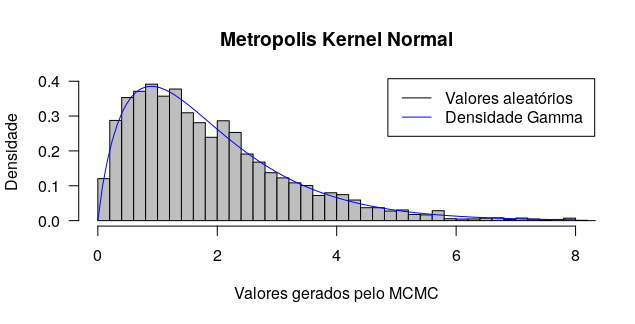
\includegraphics[width = 15cm]{MKN.png}
\end{figure}

\

\ Analogamente para figura abaixo que mostram os valores da amostra de $X$ e a curva da função $g(x)$, resultados das simulações com distribuições do núcleo uniforme com parâmetros de $inicio = 0 $ e $fim = 5$. Percebe-se que essas amostras estão condizendo com a curva, uma vez que os pontos estão distribuídos de acordo com a linha.

\begin{figure}[!htb]
\centering
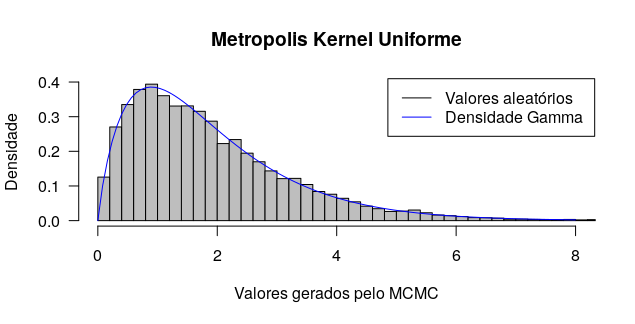
\includegraphics[width = 15cm]{MKU.png}
\end{figure}

\section{Conclusão}

\qquad A partir dos valores obtidos no cálculo da integral, podemos concluir que utilizando MCMC em problemas com funções compliciadas, é possível chegar à uma solução de uma maneira prática com uma computação relativamente simples. Porém, observei que pelo método iterativo, a sua convergência pode demorar um certo tempo, pois este EP chegou no mesmo resultado do anterior, mas não de forma instantânea.

\begin{thebibliography}{refs} % referências
\bibitem{MCMC}
        YILDIRIM, I., Bayesian Inference: Metropolis-Hastings Sampling (2012).
        \textit{Disponível em:}
        \url{http://www.mit.edu/~ilkery/papers/MetropolisHastingsSampling.pdf}.
        \textbf {acesso em 06/05/2018.}
        
\bibitem{MCMC with R}
        CHRISTIAN,C.; CASELA, G. ,Intorducing Monte Carlo Methods with R (2009).
        \textit{Disponível em:}
        \url{http://citeseerx.ist.psu.edu/viewdoc/download?doi=10.1.1.703.5878&rep=rep1&type=pdf}.
        \textbf {acesso em 09/05/2018.}
\bibitem{MC book}
		GENTLE, J.E. Statistics and Computuing. Random Number Generation and Monte Carlo Methods.$1^{st}$ edition. Fairfax. Springer. (1998). 247p.

\bibitem{for MCMC}
        STERN, J.M.,Cognitive Constructivism and the Epistemic Significance of Sharp Statistical Hypotheses in Natural Sciences(2010).
        \textit{Disponível em:}
        \url{https://www.ime.usp.br/~jstern/books/evli.pdf}.
        \textbf {acesso em 05/05/2018.}
        
\bibitem{Notas de aula}
        Notas de Aula do professor J. Stern - MAP2212 - Maio 2018       
\end{thebibliography}

\end{document}